\documentclass{article}
\usepackage{titlesec}
\usepackage[utf8]{inputenc}
\usepackage[english]{babel}
\usepackage[a4paper,pdftex,bottom=20mm, width=160mm]{geometry}
\setlength{\parindent}{0pt} 
\setlength{\parskip}{1em}
\usepackage{amsmath}
\usepackage{listings}
\usepackage{graphicx}
\usepackage{comment}
\usepackage{float}
\usepackage{biblatex}
\usepackage{lscape}
\usepackage{csquotes}
\usepackage{multirow}
\usepackage{lipsum}
\usepackage{booktabs}
\usepackage{hyperref}
\usepackage{tabularx}
\addbibresource{bib.bib}

\title{
    
\includegraphics[scale=1.5]{liu_logga.png} \\
    \vspace{2.0cm}
    \textbf{Project Management Plan} \\
    \rule{\textwidth}{0.4pt} \\
    \large \textbf{TDDC88 Programutvecklingsmetodik}
}

\author{Company 3 \\Adrian Redfors \\ Fredrik Klämmerling \\ Emma Strömberg \\ Christiana Chioma Ottona \\ Olle Lövborg}
\date{\today}

\begin{document}

\maketitle

\newpage
```latex
\section{Document Change History}

\begin{center}
\small\textit{Note: This change history table was generated by Autoleaf AI under the supervision of the Technical Writer. Only the most significant changes are highlighted, check the readme.md, found in gitlab, for more detailed information.}

\vspace{0.5cm}

\begin{tabular}{|p{0.05\textwidth}|p{0.09\textwidth}|p{0.17\textwidth}|p{0.14\textwidth}|p{0.39\textwidth}|}
\hline
\textbf{Ver.} & \textbf{Date} & \textbf{Modified Areas} & \textbf{Changed By} & \textbf{Description of Changes} \\
\hline
2.2 & 2024-10-17 & Req. Struct., User Classes, Func. Req., Non-Func. Req., Design Constraints & Analyst Team & Restructure document for clarity and traceability, introduce sub-requirements linked to main requirements, rename and restructure user roles section. Remove Software System Attributes section. \\
\hline
2.1 & 2024-10-10 & User Stories, Scope, Non-Func. Req., Overall Desc. & Analyst Team & Restructure user stories, clarify scope, streamline non-functional requirement descriptions, and improve overall description clarity. \\
\hline
2.0 & 2024-10-03 & Software Sys. Attr., User Stories, Constraints, Assumptions, Func. Req., Perf. Req. & Analyst Team & Introduce software system attributes, refine user stories, expand constraints, clarify assumptions, and provide specific details for functional and performance requirements. \\
\hline
1.1 & 2024-09-24 & Intro, Overall Desc., Specific Req. & Analyst Team & Expand initial structure with detailed descriptions of user roles, system functionalities, requirements, and constraints. \\
\hline
1.0 & 2024-09-19 & Intro, Overall Desc., Specific Req., Supporting Info & Analyst Team & Establish initial structure and content of the Requirements Specification document. \\
\hline
\end{tabular}
\end{center}

\vspace{1cm}
```
 
\newpage


\tableofcontents
\newpage


\section*{Preface}
\addcontentsline{toc}{section}{Preface}
\textit{Technical Writer Note: This document is work in progress. It demonstrates the direction we're going with the plan, it's a living document that is always in progress. Retroactive imporovements will be done.}

This document serves as the master plan for Company 3's development project in collaboration with Axis Communications AB. It outlines our systematic approach to project execution, monitoring, and control while ensuring alignment with both customer requirements and course objectives.

The Project Management Plan (PMP) defines how we organize our work across departments, manage resources, and implement key software engineering practices. It provides a comprehensive framework for:

\begin{itemize}
    \item Project process definition and control
    \item Resource allocation and monitoring
    \item Milestone planning and tracking
    \item Cross-functional team coordination
    \item Quality assurance and risk management
\end{itemize}

This document is maintained throughout the project lifecycle and serves as a reference point for all team members, linking to specialized plans such as the Quality Assurance Plan, Testing Plan, and Risk Management Plan. Regular updates will reflect our evolving understanding and improvements to our processes.

\newpage






\begin{comment}

IDESPÅN OM INNEHÅLL
Iden är att vi 


- Processes and working method (Olle)
    -The plan is to create an visual chart representing the main process in the company, in the form of the flow from requirments to a delivered product/function. This will begin the process chapter and will also includa a descriptive text written me (Olle) and the analysts.

        - Text:
            The following diagram illustrates the core process within our company for delivering a product according to customer specifications. This workflow forms the foundation of our project approach, as it provides a structured method to incorporate customer needs effectively into the final product. Consequently, any changes or adjustments to project scope are handled through this main process, as an integral part of meeting the agreed-upon specifications.
            
            The process begins with the customer submitting input on new or adjusted requirements. These requirements are first assessed by a team of analysts, who formalize them into a specification and add it to the product backlog. The requirements are then prioritized; if approved, they proceed to the development team. Otherwise, they are returned to the analysts for refinement and re-evaluation.
            
            Once the prioritized requirements are approved, they are added to the development backlog and may be broken down into smaller tasks, or subrequirements. From here, the development team implements the necessary changes, while the testing team prepares to validate the functionality. After development, testing ensures the new functionality meets quality standards. If any functionality fails the tests, it returns to the development team for adjustments. Upon successful testing, the functionality is presented to the customer for final approval.
            
            One notable limitation of this workflow is that customer satisfaction is necessary to conclude the process. If the customer is not satisfied, the feedback loop directs the process back to the analysts for a new cycle of adjustments. Only when the customer is satisfied and grants approval does the finalized version proceed to deployment. This workflow, therefore, prioritizes alignment with customer expectations over rapid completion.

        - Flow chart: Process.jpeg
            
    -After presenting the overal process, the main working methods (wich contains processes) will be reffered to according to below:
        - Testing : Test plan (https://www.overleaf.com/project/66ff9154fca1f68722259739)
        - Error handling: Described in the Testing plan, section "Bug Handling Process" (https://www.overleaf.com/project/66ff9154fca1f68722259739)
        - Handling of risks: Risk managment plan (https://www.overleaf.com/project/66e6db3848ba4493cf2e8b34)
        - Git: Described in Git (https://gitlab.liu.se/tddc88-ht24/company3/-/blob/development/README.md?ref_type=heads)
        - Change management: Is described in Quality Assurance Plan, section "Change Management"
        - Version Control (Is developed by Adrian)
        - Plan for competence and education: Is found in this document (Project Management Plan)


Management of Human Resources (Emma + Chioma)
    - Budget Management
        - Expected hours worked 
        - Burn down chart
        
    - Monitoring of people doing work 
        - Summary of time report 
        - Individual time report and action
        - Continuous coversatio about progress and time plans
        

- Milestone Plan (Fredrik)
    - Pre-iteration 1
        - Assign roles
        - Axis crash course (How to build ACAPs, connect to the hardware and use Axis documentation)
        - Identify customer needs (By interviewing representatives from Axis)
        - Organize into functional and cross-functional teams (XFT was based on Gap analysis)
        - Create high level time line (Slides to toll gate)
        - High level architecture (Changs arch. that were in the toll gate)
        - Create mockup (The Figma link: https://www.figma.com/proto/KoaRJn49T8aRgeZW0gcEv4/PanoraGuard) 
    - Iteration 1
        - Goals, Vision
            - Start developing functions and features (Tasks done by each developer team)
            - Structure requirements and connect to user stories (This excel: https://liuonline.sharepoint.com/:x:/r/sites/TDDC88_2024_C3-PnS/Delade%20dokument/Product%20and%20Sales%20%5BPnS%5D/Analysts/Product%20Backlog.xlsx?d=w1ada1d637b6f4e81870da3620dd811de&csf=1&web=1&e=fjEouW)
            - Work on Quality Assurance plan (Testers thinking about how to ensure quality)
            - Identify risks with the project (Start of risk management plan)
        - Deliverables
            - Requirements Specification
            - Quality Assurance plan
            - Risk Management plan
        - Knowledge (Fredrik skicka ett form)
            - Front end team started learning about React
        - Struktur (i organisationen)
            - Reorganize cross-functional teams based on developer divisions instead of gap analysis
        - Follow up (hur det blevs)
            Back end devs. implemented some core features
            Front end started, but was never done
            Testers started to plan testing
            Architecture was refined
            Risks were identified
            Requirements were structured
            Overall a good iteration, in next iteration - connect front and back end fully since this was not completed
    - Iteration 2
        - Goals, Vision
            - Link requirements to developement tasks and tests
            - Connect front end user interface with back end functionality, so that we have an actual website that the customer can test
                - Enable a user to log in via the UI
                - Alarms shows up in UI, with best snapshot 
            - Deploy project in Azure so that it can be accessed remotely
            - Make sure that the pipeline works as intended - testing done automatically and website built
        - Deliverables
            - Web site with basic functionality (login and alarm display)
            - Risk management
            - Document management system
        - Knowledge (Fredrik skicka ett form)
            - 2 Analysts are becoming developers and that we plan to have a dev. crash course for them
        - Struktur (i organisationen)
            - Modified cross-functional teams, now has colors instead of dev. names, updated 2 analysts converting to developers
        - Follow up (hur det blevs)
    - Iteration 3
        - Goals, Vision
            - Implement remaining back end features and connect to front end
            - Test system
            - Refine pipeline if needed
        - Deliverables
            - Web page
            - Different plans
            - Refine Rew. Spec.?
        - Knowledge 
            - No current plan 4/11-2024
        - Struktur (i organisationen)
            - If needed, covert people to developers
        - Follow up (hur det blevs)
    - Iteration 4
        - Goals, Vision
            - Buffer time
            - Complete remaining tasks
            - Ensure that we align with customer excpectation for the final release
            - Test. A lot.
        - Deliverables
            - All plans
            - The product.
        - Knowledge (Fredrik skicka ett form)
        - Struktur (i organisationen)
        - Follow up (hur det blevs)


((In med delimitations för utbildning in i SQA Plan)) 

\end{comment}



% This file is only the project Overview

\begin{comment}
    ONTENTS OF THE ENTIRE DOCUMENT
    Change History i
    Preface ii
    List of Figures v
    List of Tables vi
    1 Project Overview 1
    2 Project Overview 2
    2.1 Project Description . . . . . . . . . . . . . . . . . . . . . . . . . . . . . . . . . . . . 2
    3 Project Overview 3
    3.1 Project Description . . . . . . . . . . . . . . . . . . . . . . . . . . . . . . . . . . . . 3
    3.1.1 Background . . . . . . . . . . . . . . . . . . . . . . . . . . . . . . . . . . . . 3
    3.1.2 Scope . . . . . . . . . . . . . . . . . . . . . . . . . . . . . . . . . . . . . . . 3
    3.1.3 Purpose . . . . . . . . . . . . . . . . . . . . . . . . . . . . . . . . . . . . . . 3
    3.1.4 Objectives (SMART Goals) . . . . . . . . . . . . . . . . . . . . . . . . . . . 4
    3.2 Stakeholders . . . . . . . . . . . . . . . . . . . . . . . . . . . . . . . . . . . . . . . . 4
    3.2.1 Customer: Axis Communications AB . . . . . . . . . . . . . . . . . . . . . 4
    3.2.2 Development Team: Company 3 . . . . . . . . . . . . . . . . . . . . . . . . 4
    3.2.3 End Users . . . . . . . . . . . . . . . . . . . . . . . . . . . . . . . . . . . . . 5
    3.3 Project Constraints . . . . . . . . . . . . . . . . . . . . . . . . . . . . . . . . . . . . 5
    3.3.1 Personnel . . . . . . . . . . . . . . . . . . . . . . . . . . . . . . . . . . . . . 5
    3.3.2 Timeline . . . . . . . . . . . . . . . . . . . . . . . . . . . . . . . . . . . . . . 5
    3.3.3 Resources . . . . . . . . . . . . . . . . . . . . . . . . . . . . . . . . . . . . . 5
    3.4 Deliverables . . . . . . . . . . . . . . . . . . . . . . . . . . . . . . . . . . . . . . . . 6
    3.4.1 Product Deliverables . . . . . . . . . . . . . . . . . . . . . . . . . . . . . . . 6
    3.4.2 Documentation Deliverables . . . . . . . . . . . . . . . . . . . . . . . . . . . 6
    3.5 Project Schedule . . . . . . . . . . . . . . . . . . . . . . . . . . . . . . . . . . . . . 6
    3.5.1 Iteration Plan . . . . . . . . . . . . . . . . . . . . . . . . . . . . . . . . . . . 6
    3.5.2 Key Milestones . . . . . . . . . . . . . . . . . . . . . . . . . . . . . . . . . . 6
    3.6 Quality Objectives . . . . . . . . . . . . . . . . . . . . . . . . . . . . . . . . . . . . 7
    Vincenzo Petrone iii v1.0
    CONTENTS Project Management Plan
    3.6.1 Product Quality . . . . . . . . . . . . . . . . . . . . . . . . . . . . . . . . . 7
    3.6.2 Process Quality . . . . . . . . . . . . . . . . . . . . . . . . . . . . . . . . . . 7
    4 Project Planning 8
    4.1 Work Activities . . . . . . . . . . . . . . . . . . . . . . . . . . . . . . . . . . . . . . 8
    4.2 Time Allocation . . . . . . . . . . . . . . . . . . . . . . . . . . . . . . . . . . . . . 8
    5 Project Assessment and Control 10
    5.1 Requirements Management Plan . . . . . . . . . . . . . . . . . . . . . . . . . . . . 10
    5.2 Scope Change Control Plan . . . . . . . . . . . . . . . . . . . . . . . . . . . . . . . 10
    5.3 Schedule Control Plan . . . . . . . . . . . . . . . . . . . . . . . . . . . . . . . . . . 11
    5.4 Budget Control Plan . . . . . . . . . . . . . . . . . . . . . . . . . . . . . . . . . . . 11
    5.5 Quality Assurance Plan . . . . . . . . . . . . . . . . . . . . . . . . . . . . . . . . . 11
    5.6 Dissemination Plan . . . . . . . . . . . . . . . . . . . . . . . . . . . . . . . . . . . . 12
    5.6.1 Scientific dissemination . . . . . . . . . . . . . . . . . . . . . . . . . . . . . 12
    5.6.2 General-purpose dissemination . . . . . . . . . . . . . . . . . . . . . . . . . 12
    6 Supporting Process Plans 13
    6.1 Risk Management . . . . . . . . . . . . . . . . . . . . . . . . . . . . . . . . . . . . 13
    6.1.1 Negative risks . . . . . . . . . . . . . . . . . . . . . . . . . . . . . . . . . . . 13
    6.1.2 Positive risks . . . . . . . . . . . . . . . . . . . . . . . . . . . . . . . . . . . 14
    6.2 Cost Management . . . . . . . . . . . . . . . . . . . . . . . . . . . . . . . . . . . . 14
    Acronyms 15
    References 16
    
\end{comment}
    
    
    
    

\section{Project Overview}
\subsection{Project Description}
    
\subsubsection{Background}
As part of the TDDC88 Software Engineering Theory and Practice course at Linköping University, Company 3 has been tasked with developing a software solution for Axis Communications AB. This project aims to create PanoraGuard; a system for interpreting and analyzing streamed or recorded video content, with a specific focus on security surveillance.
    
\subsubsection{Scope}
The project encompasses the development of a functional prototype that demonstrates advanced capabilities in video analysis for security surveillance. Our system, PanoraGuard, will integrate with Axis camera systems to provide real-time object recognition and motion detection. It will process video data to identify potential security threats, alerting operators to unauthorized access in specified areas. The scope includes developing a user-friendly interface for monitoring and control, allowing security personnel to make informed decisions quickly. While our focus is on software development, we will ensure seamless integration with Axis hardware. The project does not include hardware development or large-scale deployment but will provide a robust foundation for future scalability.
    
\subsubsection{Purpose}
The primary purpose of this project is twofold:
\begin{enumerate}
    \item To create a demonstrable product of value for Axis Communications that addresses their real-world needs in video analytics for security applications.
    \item To provide Company 3 members with practical experience in large-scale software engineering, from initial concept to final delivery, mirroring real-world development processes.
\end{enumerate}
    
\subsubsection{Objectives (SMART Goals)}
\begin{enumerate}
    \item \textbf{Specific:} Develop a working prototype of PanoraGuard capable of detecting and alerting unauthorized access in specified areas by the end of Iteration 3 (November 22, 2024).
    \item \textbf{Measurable:} Implement core features including motion detection, object recognition, and an alert system with a 95\% accuracy rate by the end of Iteration 2 (November 8, 2024).
    \item \textbf{Agreed:} Achieve full alignment with Axis Communications' requirements and TDDC88 course objectives, as confirmed in the Tollgate meeting on September 26, 2024.
    \item \textbf{Realistic:} Complete development within the 160-hour active work time per team member constraint, utilizing our cross-functional team structure for efficient resource allocation and task completion.
    \item \textbf{Timely:} Deliver a fully functional PanoraGuard prototype, complete with user interface and integration capabilities, for presentation at VSSE'24 on December 12, 2024.
\end{enumerate}
    
Our team is committed to creating a system that not only meets the technical requirements but also provides an intuitive, seamless user experience for security operators. By focusing on rapid alert systems, clear visual interfaces, and robust backend processing, PanoraGuard aims to set a new standard in video-based security surveillance.
    
\subsection{Stakeholders}
    
\subsubsection{Customer: Axis Communications AB}
Axis Communications AB, the primary stakeholder and customer, is a leader in network video solutions. They provide the hardware infrastructure and industry expertise that our software solution will complement. Axis requires a video analysis system for security surveillance that integrates with their camera systems. Key requirements include real-time threat detection, alert mechanisms, and an interface for security operators, all compliant with industry standards and data protection regulations.
    
\subsubsection{Development Team: Company 3}
Company 3 consists of students from the TDDC88 course, organized into functional groups and cross-functional teams for efficient development. The functional group structure includes:
    
\begin{description}
    \item[Management:] Overseeing project timeline, resource allocation, and communication.
    \item[Architecture:] Designing system structure and integration points.
    \item[Development:] Creating user interfaces and implementing core functionalities.
    \item[Quality Assurance and Testing:] Ensuring software reliability and performance.
    \item[UX/UI Design:] Optimizing user experience for security personnel.
    \item[Analysis:] Evaluating system performance and user needs.
    \item[Deployment:] Managing system integration and rollout. 
\end{description}
    
The company is organized into four cross-functional units: ACAP, LAN SERVER, CLIENT, and EXTERNAL. Each unit combines various roles from the functional structure to address specific aspects of the project, promoting collaboration and efficient problem-solving. The corss-functional teams can be shown in the figure below.

\begin{figure}[h]
    \centering
    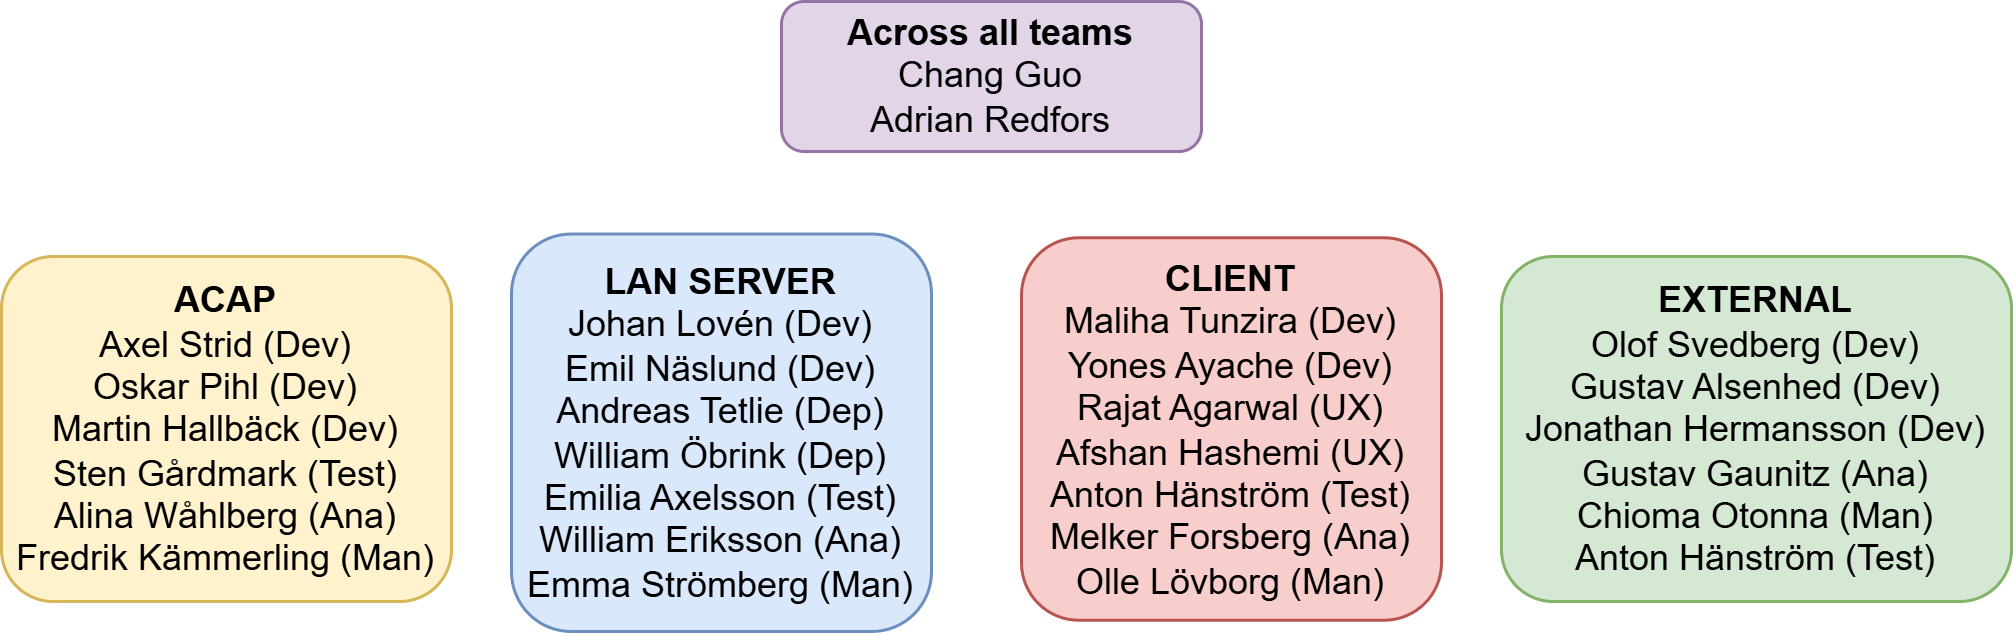
\includegraphics[width=0.5\linewidth]{NewCrossFunctional.drawio.png}
    \caption{Cross-functional teams for Iteration 1 \& 2}
    \label{fig:enter-label}
\end{figure}
    
\subsubsection{End Users}
The primary end users require efficient alert systems, clear data visualizations, and intuitive controls for managing security incidents. These users of the system will be security professionals, including:
    
\begin{itemize}
    \item Security operators monitoring video feeds and responding to alerts
    \item Security managers overseeing operations and accessing analytical data
    \item System administrators managing access and configurations
\end{itemize}
    

    
\subsection{Project Constraints}
    
\subsubsection{Personnel}
The project is constrained by a 160-hour limit per team member. This necessitates careful planning and resource management throughout the project lifecycle. Additionally, team members have other academic commitments inherent to being students, which must be respected and managed alongside project work. This differs from a traditional work environment and requires flexible scheduling and efficient time utilization.
    
\subsubsection{Timeline}
The timeline of the project requires management of development cycles and regular progress reviews to ensure in-time delivery of project milestones. The project is bound by the following key dates:
    
\begin{tabular}{ll}
    \textbf{Event} & \textbf{Date} \\
    \hline
        Project Start & September 4, 2024 \\
        Tollgate Meeting & September 26, 2024 \\
        Iteration 1 End & October 11, 2024 \\
        Iteration 2 End & November 8, 2024 \\
        Iteration 3 End & November 22, 2024 \\
        Iteration 4 End & December 6, 2024 \\
        VSSE (Final Presentation) & December 12, 2024 \\
\end{tabular}

    
\subsubsection{Resources}
The project operates without a dedicated budget, which significantly impacts available resources. Key constraints include:
    
\begin{itemize}
    \item Reliance on virtual environments for large-scale testing scenarios
    \item No funds for third-party software licenses, AI models, or cloud computing resources
    \item Time constraints for students in our company
    \item Time limitations for learning new technologies or frameworks
\end{itemize}
    
To address these constraints, the team will focus on open-source tools, efficient resource utilization, and prioritization of core functionalities. Open communication with Axis Communications and the course adminstration will be maintained for any critical support or resources needed for project success.

\subsubsection{Competence Plan}
To ensure effective use of the resources in the company a competence plan has been made. This includes providing various learning tools to enhance team competence. These resources include:
\begin{itemize}
    \item \textbf{Course material} - labs, lectures, and exercises from course materials available and attended to all company members.
    \item \textbf{Company lectures} - One introduction to C was held by Magnus Nielsen, but this was the only lecture expressively needed by the development team.
    \item \textbf{Self-learning modules} - the main method of competence development is individual. This is to encourage continuous development and estimation of what the individual needs to execute their respective task.
    \item \textbf{Education tag in Planner} - operation to track and give an overview of knowledge in the company. 
\end{itemize}

Through the plan, each team member and group is encouraged to proactively anticipate their future learning needs. This may involve diverse knowledge areas, such as requirements gathering, testing, traceability, integration, deployment in Docker or Azure, and more.

To maintain a clear record of the knowledge within the company, all employees are encouraged to log their learning and assignments as tasks in our project planner. By tagging these entries with "education," we can trace and reference the expertise within the company for future reuse.

\subsubsubsection{Gap Analysis}
To have an initial understanding of the existing competence in the company, a gap analysis was performed using \textit{assignments} through Microsoft Teams. This analysis focused on key areas of knowledge, particularly in "programming" and "git." Skills were assessed using the following levels:

\begin{itemize}
    \item \textbf{Level 1 – Assists}: Basic understanding of the concepts and the ability to follow instructions.
    \item \textbf{Level 2 – Applies}: Can apply the concepts in simple contexts by routinely using prior experience.
    \item \textbf{Level 3 – Masters}: Can apply the concepts in most contexts and has the experience to work without supervision.
    \item \textbf{Level 4 – Adapts}: Possesses judgment on when and how to apply the concepts in more complex contexts. Can enable others to apply the concepts.
    % \item \textbf{Level 5 – (optional)}: Please check lecture notes for any additional levels.
\end{itemize}

\subsubsubsection{Onboarding New Groups and Team Members}
When a new team member joins or an existing employee is assigned to a new role, onboarding procedures include:
\begin{itemize}
    \item Assignment to a cross-functional team for active participation.
    \item Assignment of mentors to facilitate the transition into the new role.
\end{itemize}

Special considerations are given to the remaining project time for relocated employees relative to the average time remaining for other team members. For example, analysts transitioning into developer roles with less time left are given tasks that are either less time-consuming or fewer in number.

If additional resources are required for a functional group, the project manager decides on personnel redistribution. Line managers, with input from the group, make employees available as needed. This process is primarily used when re-distributing roles. 

\subsubsubsection{Follow-up}
To assess the effectiveness of this competence plan, a poll will be conducted at the end of iteration 2. Employees will be asked if they feel adequately equipped with the knowledge required to complete their tasks, whether the self-learning approach has been beneficial, and if there are specific areas where further training would be helpful. A poll is exemplified in Image \ref{fig:competence_follow_up}
 below.

 \begin{figure}[h]
     \centering
     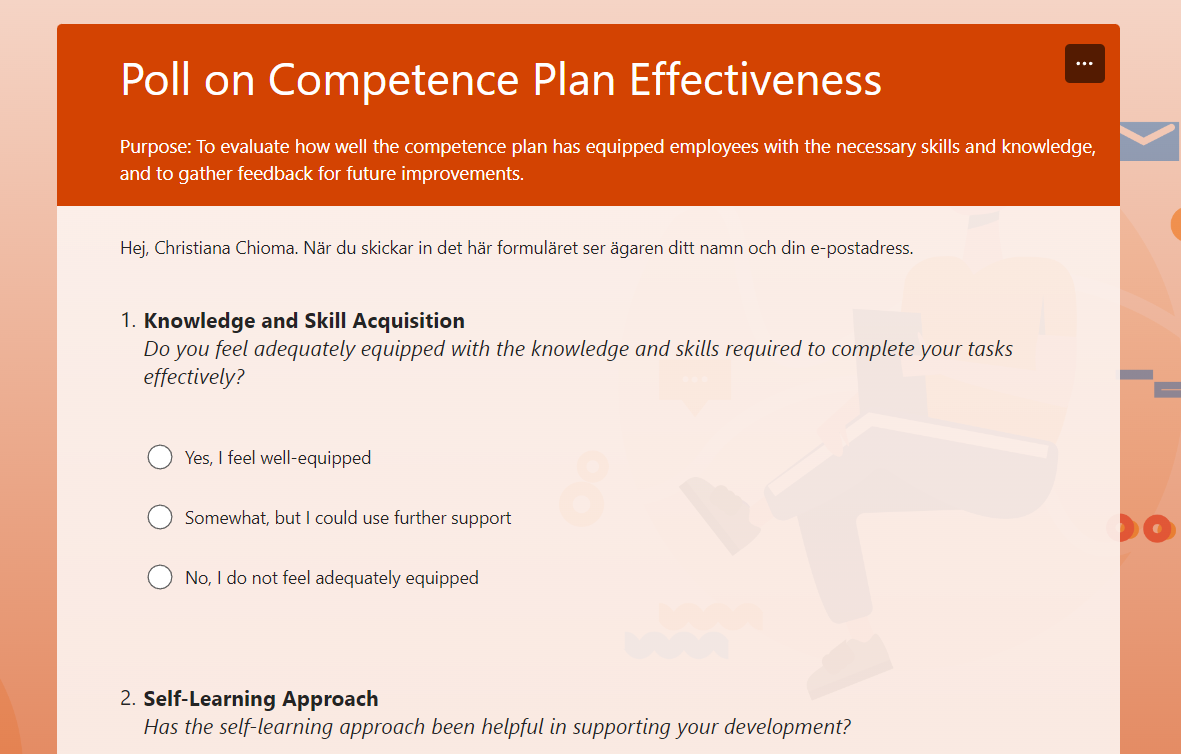
\includegraphics[width=0.75\linewidth]{competence_follow_up.png}
     \caption{Poll for follow-up of company competence.}
     \label{fig:competence_follow_up}
 \end{figure}

    
\subsection{Deliverables}
The project will result in both product and documentation deliverables, each crucial to the success of the security surveillance solution.
    
\subsubsection{Product Deliverables}
    
The core of our solution will comprise of several connected components:
    
   % @Chioma, please confirm the deliverables from development team
\begin{description}
    \item[Video Analysis Engine:] For processing video feeds and detecting anomalies. (this has to be parapharased to acurately match wht the goals are otherwise the rest checks out.. il get back to this // chioma
    \item[Alert Management System:] For generating and managing security alerts.
    \item[Operator Interface:] A dashboard for security personnel to monitor and respond to alerts.
    \item[Camera Integration Module:] For integration with Axis camera systems.
    % \item[Data Visualization Tool] Need to confirm if this is a required component
\end{description}
    
    % Additional components may be needed based on specific project requirements - Fredrik Kämmerling?
    
\subsubsection{Documentation Deliverables}

To support our product and ensure its proper implementation and use, we will produce the following key documents:

\begin{center}
\begin{tabular}{|p{0.3\textwidth}|p{0.6\textwidth}|}
    \hline
    \textbf{Document} & \textbf{Description} \\
    \hline
    Architecture Notebook & Overview of system architecture and design rationale \\
    \hline
    Project Backlog & Listing of functional and non-functional system requirements \\
    \hline
    Test Plan & Outline of testing strategies and procedures \\
    \hline
    Software Quality Assurance Plan & Documentation of quality standards and processes \\
    \hline
    Customer Requirements Specification & Documentation of customer requirements and expectations \\
    \hline
\end{tabular}
\end{center}

\section{Project Schedule}

Our project timeline is structured to ensure steady progress and regular delivery of value. Work is divided into four key iterations.

\subsubsection{Iteration Plan}
Presented below are the dates and focus areas of each iteration: 
\begin{center}
    \begin{tabular}{|c|l|l|}
        \hline
        \textbf{Iteration} & \textbf{Dates} & \textbf{Focus} \\
        \hline
        0 (Tollgate) & Sept 13 - Sept 26 & Company Overview, Requirements Specification, Architectural Description, Milestone Plan, Acceptance Testing Plan, UX \& Organizational Structure \\
        \hline
        1 & Sept 30 - Oct 11 & System Integration, Database Setup, Initial Client-Facing Website Development, SQA Plan, Test Plan, CI/CD Plan \\
        \hline
        2 & Oct 14 - Nov 8 & Alarm Management, Scheduling System Development, Continued Client-Facing Website Development \\
        \hline
        3 & Nov 11 - Nov 22 & Continued Scheduling System Development, Alarm Confidence Level, Multi-Camera Support \\
        \hline
        4 & NOv 22 - Dec 6 & Data Compliance \& GDPR Management, Scalability Enhancement, Final Presentation Preparation \\
        \hline
    \end{tabular}
    \end{center}


\subsubsection{Key Milestones}

Our project timeline contains the following key events:

\begin{center}
\begin{tabular}{|l|c|}
    \hline
    \textbf{Milestone} & \textbf{Date} \\
    \hline
    Project Kickoff & September 4, 2024 \\
    Tollgate Meeting & September 26, 2024 \\
    Iteration 1 End & October 11, 2024 \\
    Iteration 2 End & November 8, 2024 \\
    Iteration 3 End & November 22, 2024 \\
    VSSE (Final Presentation) & December 12, 2024 \\
    \hline
\end{tabular}
\end{center}


\begin{figure}[h]
    \centering
    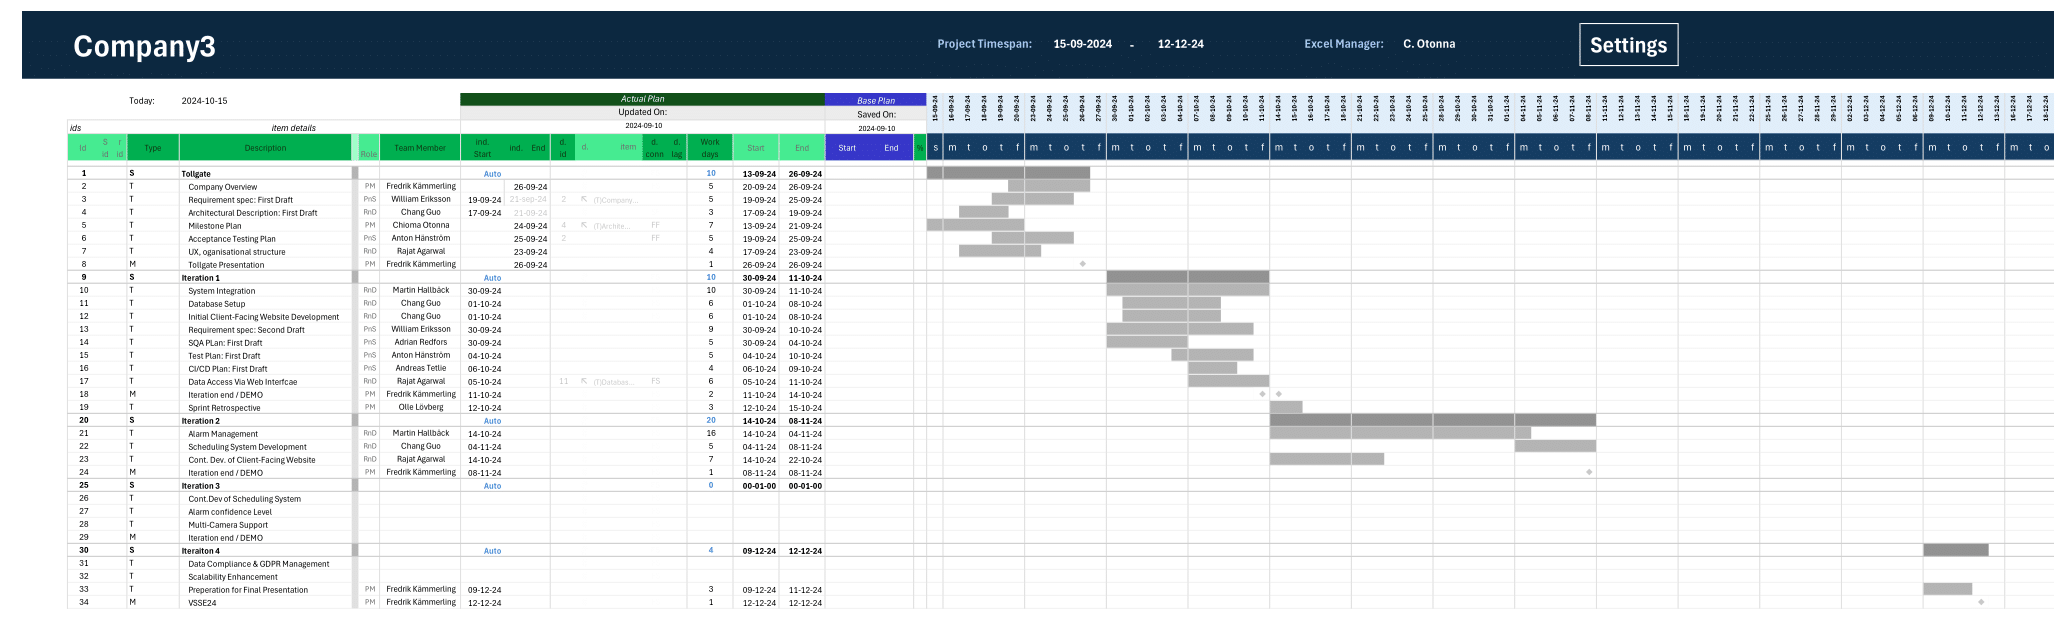
\includegraphics[width=\textwidth]{Milestone Plan-1.png}
    \caption{Project Milestone Plan and Gantt Chart}
    \label{fig:milestone-plan}
\end{figure}
%additional pitcure of the milestone plan / iteration plan in the begining of the project is needed.  /chioma - i will provide. 

\subsection{Quality Objectives}

Quality is at the heart of our development process, encompassing both the product we deliver and the methods we employ to create it.

\subsubsection{Product Quality}

Our security surveillance solution aims to meet the following quality benchmarks:

% Need to confirm specific quality metrics with stakeholders
% @Emma: Please confirm the quality metrics
\begin{itemize}
    \item Achieve high system uptime during operational hours.
    \item Generate alerts within a specified time frame of incident detection.
    \item Maintain a low false positive rate for security alerts.
    \item Design an intuitive interface for efficient user interaction.
    \item Support multiple simultaneous camera feeds.
\end{itemize}


\subsubsection{Process Quality}

% @Chioma: Please confirm the rnd side of things here 
To ensure an effective development process, we commit to:

Adhering to iterative development methodologies, with regular reviews and retrospectives to continuously improve our processes. Our documentation will be updated at the conclusion of each iteration to reflect the latest project state.

Implementing a comprehensive Quality Assurance plan that is iterative in nature, with a focus on continuous improvement. This plan spans across both the Research and Development (RnD) and Product and Sales (PnS) departments, covering all iterations. Key roles and responsibilities are outlined in Table \ref{tab:qa-responsibilities}.

\begin{table}[h]
\centering
\caption{Quality Assurance Roles and Responsibilities}
\label{tab:qa-responsibilities}
\begin{tabular}{|l|l|}
\hline
\textbf{Role} & \textbf{Responsibility} \\
\hline
Product and Sales Line Manager & Overall QA plan \\
Technical Writer & Document structure and version control \\
Testing Lead & Testing strategy and bug tracking \\
Analysis Lead & Traceability \\
Deployment Lead & Continuous integration and delivery \\
Process Manager & Internal quality practices and change management \\
Architecture & Future development and operations considerations \\
\hline
\end{tabular}
\end{table}

Utilizing a Continuous Integration and Continuous Delivery (CI/CD) pipeline to automate the build, test, and deployment processes. Our CI/CD pipeline, managed through GitLab CI, includes automated testing, Docker image building, and deployment to a Kubernetes cluster hosted in Azure. This approach ensures consistent code quality, frequent integration, and reliable deployments.

Maintaining code quality through review processes before merging major features into our main codebase. We aim for comprehensive automated testing coverage for all new code, ensuring reliability.

Soliciting regular stakeholder feedback, with dedicated sessions throughout the project. This approach ensures that we remain aligned with stakeholder expectations and can adapt to changing requirements or priorities.

Conducting sprint retrospectives after each iteration to evaluate our practices and processes, as outlined in our quality management plan. These retrospectives will cover areas such as document version handling, internal test cases, code refactoring, methods of communication, and the retrospective process itself.

Implementing a feedback loop system where all employees are encouraged to provide continuous feedback and recommendations on quality assurance practices to their Lead, Line Manager, or the Project Manager.

Through these quality objectives and processes, we aim to deliver a security surveillance solution that maintains high standards of quality throughout its development lifecycle.
\begin{comment}
    - Processes and working method (Olle)
    -The plan is to create an visual chart representing the main process in the company, in the form of the flow from requirments to a delivered product/function. This will begin the process chapter and will also includa a descriptive text written me (Olle) and the analysts. (OLLE DOES THIS)

    -After presenting the overal process, the main working methods (wich contains processes) will be reffered to according to below:
        - Testing : Test plan (
        - Error handling: Described in the Test plan (
        - Handling of risks: Risk managment plan (https://www.overleaf.com/project/66e6db3848ba4493cf2e8b34)
        - Git: Described in Git (https://gitlab.liu.se/tddc88-ht24/company3/-/blob/development/README.md?ref_type=heads)
        - Change management: Is described in Quality Assurance Plan, section "Change Management"
        - Version Control (Is developed by Adrian)
        - Plan for competence and education: Is found in this document (Project Management Plan)

LINKS
 https://liuonline.sharepoint.com/:u:/r/sites/TDDC88_2024_C3/Delade%20dokument/General/Output/Link%20to%20Git/Customer%20Requirements%20Specification.url?csf=1&web=1&e=cVdXEu
 
 https://liuonline.sharepoint.com/:u:/r/sites/TDDC88_2024_C3/Delade%20dokument/General/Output/Link%20to%20Git/Customer%20Requirements%20Specification.url?csf=1&web=1&e=cVdXEu
 
 https://liuonline.sharepoint.com/:u:/r/sites/TDDC88_2024_C3/Delade%20dokument/General/Output/Link%20to%20Git/Project%20Managment%20Plan.url?csf=1&web=1&e=j1VKkT
 
 https://liuonline.sharepoint.com/:u:/r/sites/TDDC88_2024_C3/Delade%20dokument/General/Output/Link%20to%20Git/Quality%20Assurance%20Plan.url?csf=1&web=1&e=LBJMch
 
 https://liuonline.sharepoint.com/:u:/r/sites/TDDC88_2024_C3/Delade%20dokument/General/Output/Link%20to%20Git/Risk%20Managment%20Plan.url?csf=1&web=1&e=OS3l2q
 
 https://liuonline.sharepoint.com/:u:/r/sites/TDDC88_2024_C3/Delade%20dokument/General/Output/Link%20to%20Git/Testing%20Plan.url?csf=1&web=1&e=hVyQSJ


\end{comment}




\section{Processes and Working Methods}

The development processes in Company 3 follow an iterative structure designed to align with the project's four iterations. This section provides an overview of the main processes and references to their detailed documentation.

\begin{figure}[h]
    \centering
    % TODO: Insert process flow diagram
    \caption{Development Process Flow}
    \label{fig:process-flow}
\end{figure}

% Version Control placeholder 
\subsection*{Version Control Strategy}
Version control for project documentation follows a semi-automated approach integrating Overleaf and GitLab repositories. The process is managed through a custom utility tool that handles version tracking and changelog generation.

\subsubsection*{Documentation Flow}
The version control process consists of the following steps:
\begin{enumerate}
    \item Documents are primarily edited in the Overleaf collaborative environment
    \item The custom utility tool:
    \begin{itemize}
        \item Clones Overleaf repositories
        \item Generates an updated changelog for each document
        \item Creates a readme file along with a \texttt{version\_control.tex} file documenting the latest version updates
        \item Updates the version control page following each document's title page
    \end{itemize}
    \item Generated PDFs and their corresponding repositories are uploaded to GitLab along with updated readme files
\end{enumerate}

This centralized approach reduces manual documentation overhead while maintaining consistent version tracking across project documentation. The system enables transparent tracking of document evolution and ensures both current and historical document versions remain accessible through GitLab.

\subsection*{Process Documentation}
The table below maps key processes to their documentation:

\begin{table}[h]
\begin{tabularx}{\textwidth}{>{\raggedright\arraybackslash}p{0.25\textwidth}>{\raggedright\arraybackslash}X}
\toprule
\textbf{Process Area} & \textbf{Documentation Reference} \\
\midrule
Testing \& Error Handling & \href{https://gitlab.liu.se/tddc88-ht24/company3/-/raw/Doc\_Version\_Control/Documentation/Testing\%20Plan/Testing\_Plan.pdf?ref\_type=heads\&inline=false}{Testing Plan} (Section 3.2: Bug Handling Process) \\
\addlinespace
Risk Management & \href{https://gitlab.liu.se/tddc88-ht24/company3/-/raw/Doc\_Version\_Control/Documentation/Risk\%20Management\%20Plan/Risk\_Management\_Plan.pdf?ref\_type=heads\&inline=false}{Risk Management Plan} \\
\addlinespace
Git Workflow & \href{https://gitlab.liu.se/tddc88-ht24/company3/-/blob/development/README.md?ref\_type=heads}{Project Repository README} \\
\addlinespace
Change Management & \href{https://gitlab.liu.se/tddc88-ht24/company3/-/raw/Doc\_Version\_Control/Documentation/Software\%20Quality\%20Assurance/Quality\_Assurance\_Plan.pdf?ref\_type=heads\&inline=false}{Quality Assurance Plan} (Section 9) \\
\addlinespace
Competence Development & Section 4.4: Competence Plan (this document) \\
\bottomrule
\end{tabularx}
\caption{Process Documentation Reference}
\label{tab:process-docs}
\end{table}

Each document listed above serves as the primary reference for its respective process area. Updates to processes are managed through the change management procedures outlined in the Quality Assurance Plan.
\section{Management of Human Resources}

\textit{Note from Emma: The structure below reflects our current approach to resource management, incorporating both strategic and operational perspectives. Currently compiling metrics from our tracking systems.}

\subsection{Budget Management}
Our budget management framework centers on the effective allocation and tracking of the 160-hour project budget per team member. This systematic approach ensures optimal resource utilization while maintaining project momentum.

\begin{figure}[H]
    \centering
    \includegraphics[width=0.8\textwidth]{placeholder}
    \caption{Project Hours Burn Down Chart}
    \label{fig:burndown}
\end{figure}

\textit{Chioma: Adding current burn down data from last week's department reports. Graph will show tracked hours against ideal burn down line.}

\subsubsection{Expected Hours Worked}
\textit{Adrian: Placeholder Data, updating with real numbers asap}
Current tracking indicates:

\begin{table}[H]
\begin{tabularx}{\textwidth}{>{\raggedright\arraybackslash}X>{\centering\arraybackslash}p{3cm}>{\centering\arraybackslash}p{3cm}}
\toprule
\textbf{Project Phase} & \textbf{Expected Hours} & \textbf{Actual Hours} \\
\midrule
Pre-study & 20 & 22.5 \\
Iteration 1 & 40 & 38.7 \\
Iteration 2 & 40 & 41.2 \\
\textit{Iteration 3} & \textit{40} & \textit{In progress} \\
\textit{Iteration 4} & \textit{20} & \textit{Planned} \\
\bottomrule
\end{tabularx}
\caption{Hour Distribution by Project Phase}
\label{tab:hour-distribution}
\end{table}



\subsection{Resource Monitoring}
\subsubsection{Time Report Summary}

\begin{itemize}
    \item Weekly time reports submitted through Teams
    \item Department-level aggregation by managers
    \item Individual progress tracking through GitLab activity
\end{itemize}

\textit{Chioma & Adrian: Expanding this section with specific monitoring KPIs}

\subsubsection{Progress Monitoring Framework}
Our established monitoring cadence includes:

\begin{table}[H]
\begin{tabularx}{\textwidth}{>{\raggedright\arraybackslash}X>{\raggedright\arraybackslash}X}
\toprule
\textbf{Activity} & \textbf{Frequency} \\
\midrule
Department Sync & Weekly (Thursdays) \\
Individual Updates & Bi-weekly \\
Status Reports & Weekly (Mondays) \\
Resource Review & Monthly \\
\bottomrule
\end{tabularx}
\caption{Monitoring Schedule}
\label{tab:monitoring-schedule}
\end{table}

\textit{Adrian: Adding integration points with our risk management process. Will reference specific sections from Risk Management Plan.}

\subsection{Action Planning}
Current focus areas:
\begin{itemize}
    \item Resource utilization optimization
    \item Cross-functional team balance
    \item Skill development tracking
\end{itemize}

\textit{Note from Technical Writer: Incorporating latest metrics from iteration 2 retrospective. Section will link to specific examples of implemented actions.}
\section{Project Milestone Plan}

\textit{Technical Writer Note: Standardizing section formats across iterations and adding cross-references to relevant documents.}

\begin{figure}[t!]
\centering
\includegraphics[width=0.9\textwidth]{placeholder}
\caption{Project Timeline Overview}
\label{fig:timeline}
\end{figure}

The project follows a structured approach across four iterations, with a preceding pre-iteration phase. Each phase maintains consistent tracking of goals, deliverables, knowledge development, and organizational structure.

\textit{Fredrik: Adding quantitative data from our tracking systems to support the documented progress.}

\subsection*{Phase Overview}
\addcontentsline{toc}{subsection}{Phase Overview}
\begin{table}[h!]
\begin{tabularx}{\textwidth}{>{\raggedright\arraybackslash}X>{\raggedright\arraybackslash}X}
\toprule
\textbf{Phase} & \textbf{Key Focus} \\
\midrule
Pre-Iteration & Foundation \& Planning \\
Iteration 1 & Core Development Initiation \\
Iteration 2 & System Integration \\
Iteration 3 & Feature Completion \\
Iteration 4 & Quality Assurance \\
\bottomrule
\end{tabularx}
\caption{Project Phase Overview}
\label{tab:phase-overview}
\end{table}

\subsection{Pre-Iteration Phase}
\noindent\rule{\textwidth}{0.4pt}

The pre-iteration phase established our project foundations through systematic role assignments and initial team organization. Team members participated in the Axis crash course, gaining familiarity with ACAP development, hardware connections, and documentation systems. 

Customer needs were gathered through direct interviews with Axis representatives. Initial team organization implemented Gap Analysis principles for cross-functional team formation. The tollgate meeting presented our high-level timeline alongside Chang's architecture overview. User interface concepts were visualized through our PanoraGuard Figma prototype.

\subsection{Iteration 1}
\noindent\rule{\textwidth}{0.4pt}

\subsubsection*{Goals and Vision}
\addcontentsline{toc}{subsubsection}{Goals and Vision}
The first iteration centered on initiating core development activities. Development teams began implementing initial functions while analysts worked on structuring requirements and connecting them to user stories. The testing team started formulating the Quality Assurance plan, while parallel work began on identifying and documenting project risks.

\subsubsection*{Deliverables}
\addcontentsline{toc}{subsubsection}{Deliverables}
This iteration produced three foundational documents: the Requirements Specification, Quality Assurance plan, and Risk Management plan. Each document underwent initial review cycles and established baseline versions for future refinement.

\begin{center}
\noindent\fbox{\begin{minipage}{0.97\textwidth}
\textbf{Knowledge Development:} The front-end development team engaged in React training, establishing the technical foundation for our user interface implementation.
\end{minipage}}
\end{center}

\subsubsection*{Organizational Structure}
\addcontentsline{toc}{subsubsection}{Organizational Structure}
Our organizational approach evolved from the initial Gap Analysis structure to a developer division-based arrangement of cross-functional teams. This adjustment aimed to optimize development workflows and team communication.

\subsection{Iteration 2}
\noindent\rule{\textwidth}{0.4pt}

\subsubsection*{Goals and Vision}
\addcontentsline{toc}{subsubsection}{Goals and Vision}
The second iteration prioritized system integration. Work focused on connecting requirements to development tasks and establishing links between frontend and backend components. Key objectives included implementing user authentication, displaying alarms with snapshots, and deploying the system to Azure. Pipeline implementation became a central focus for ensuring automated testing and build processes.

\begin{center}
\noindent\fbox{\begin{minipage}{0.97\textwidth}
\textbf{Integration Milestones:}
\vspace{1mm}
\begin{description}
\item[Frontend-Backend Connection] User authentication and alarm display
\item[Deployment] Azure infrastructure setup
\item[Pipeline] Automated testing and build system
\end{description}
\end{minipage}}
\end{center}

\subsubsection*{Knowledge Development}
\addcontentsline{toc}{subsubsection}{Knowledge Development}
Two analysts began their transition to development roles through a structured developer training program.

\textit{Fredrik: Adding concrete outcomes from iteration 2 as they are finalized.}

\subsection{Iteration 3 - Current Phase}
\noindent\rule{\textwidth}{0.4pt}

Our current iteration focuses on completing remaining back-end features and their integration with the front-end components. System testing has moved to the forefront of activities, with pipeline refinement continuing as needed based on development requirements.

\vspace{0.5cm}
\begin{center}
\begin{tabular}{|p{0.45\textwidth}|p{0.45\textwidth}|}
\hline
\multicolumn{2}{|c|}{\textbf{Current Focus Areas}} \\
\hline
Back-end Feature Completion & Front-end Integration \\
System Testing Implementation & Pipeline Refinement \\
\hline
\end{tabular}
\end{center}
\vspace{0.5cm}

\subsection{Iteration 4 - Planned}
\noindent\rule{\textwidth}{0.4pt}

The final iteration will serve as a buffer period for completing remaining tasks and ensuring alignment with customer expectations. Testing activities will intensify to ensure product quality meets release standards.

\begin{center}
\noindent\fbox{\begin{minipage}{0.97\textwidth}
\textbf{Final Phase Objectives}
\vspace{1mm}

Quality assurance and testing completion, with focus on customer acceptance criteria. Documentation finalization and product release preparation.
\end{minipage}}
\end{center}



\newpage
\printbibliography
\end{document}
